\documentclass[12pt]{article}
\usepackage[english]{babel}
\usepackage[a4paper, total={6in, 8in}]{geometry}
\usepackage[utf8]{inputenc}
\usepackage{graphicx}
\usepackage{algorithm}
\usepackage[noend]{algpseudocode}
\usepackage{caption}

\makeatletter

\newenvironment{breakablealgorithm}
  {% \begin{breakablealgorithm}
   \begin{center}
   \refstepcounter{algorithm}
   \hrule height.8pt depth0pt \kern2pt
   \renewcommand{\caption}[2][\relax]{%
     {\raggedright\textbf{\ALG@name~\thealgorithm} ##2\par}%
     \ifx\relax##1\relax
       \addcontentsline{loa}{algorithm}{\protect\numberline{\thealgorithm}##2}%
     \else
       \addcontentsline{loa}{algorithm}{\protect\numberline{\thealgorithm}##1}%
     \fi
     \kern2pt\hrule\kern2pt
   }}
  {% \end{breakablealgorithm}
   \kern2pt\hrule\relax
   \end{center}
  }
\makeatother

\usepackage[title]{appendix}

\usepackage[most]{tcolorbox}
\newtcolorbox{mybox2}{colback=cyan!30!white,colframe=cyan!30!white}
\newtcolorbox{mybox3}{
  breakable,
  colback=black!10!white,
  colframe=black!10!white
}

\usepackage{marginnote}
\setlength{\marginparwidth}{2.2cm}
\newcommand{\coauthortodo}[1]{%
  \marginnote{%
    \begin{tcolorbox}[
      width=\marginparwidth,
      colback=yellow!15!white, colframe=orange!70!black,
      colbacktitle=yellow!35!white, coltitle=black,
      title=TODO, fonttitle=\bfseries\scriptsize,
      toptitle=2pt, bottomtitle=2pt,
      fontupper=\scriptsize, boxrule=0.4pt, arc=1mm,
      boxsep=0pt, left=2pt, right=2pt, top=3pt, bottom=3pt,
      before skip=0pt, after skip=0pt
    ]
      \raggedright #1
    \end{tcolorbox}%
  }%
}

\usepackage{booktabs}
\usepackage[round,authoryear]{natbib}
\bibliographystyle{apalike}

\usepackage{tikz}
\usetikzlibrary{positioning}
\tikzset{
  nodecircle/.style={circle,draw,minimum size=8mm,inner sep=0pt},
  ld/.style={thick},
  dif/.style={->,thick},
  scoreedge/.style={thick,densely dotted},
  removed/.style={thick,dashed,red},
  kept/.style={thick,blue}
}

\usepackage{amsmath}
\usepackage{amssymb}
\usepackage{amsthm}

\def\s{\ensuremath\sigma}
\def\b{\ensuremath\beta}
\def\t{\ensuremath\theta}
\def\l{\ensuremath\lambda}

% Define the hollow circle used to mark the end of an Example
\newcommand{\exampleend}{\hfill\tikz\draw (0,0) circle (1.2pt);}

\newtheoremstyle{examplestyle}
  {10pt}    % Space above
  {10pt}    % Space below
  {\normalfont}  % Body font
  {}        % Indent amount
  {\bfseries}   % Theorem head font
  {.}       % Punctuation after theorem head
  {1em}     % Space after theorem head
  {}        % Theorem head spec (can be left empty, meaning 'normal')

\theoremstyle{examplestyle}
\newtheorem{example}{Example}[section]

\usepackage{etoolbox}
\AtEndEnvironment{example}{\exampleend}

\usepackage{float}
\usepackage{authblk}

\usepackage[hidelinks]{hyperref}

\title{Item screening in graphical Rasch models: a tutorial}
\author{Sebastian Kvist, Karl Bang Christensen \& Andreas Kryger Jensen}
\affil{Section of Biostatistics, Department of Public Health, University of Copenhagen}
\date{\today}

\begin{document}

\maketitle

\begin{abstract}
Rasch models are widely used to analyze questionnaire and test data. Inference based on the standard Rasch model requires assumptions such as local independence and the absence of differential item functioning. Graphical Rasch models provide a framework in which these departures can be represented explicitly. In this context, ``item screening'' denotes a coherent workflow that checks consistency, screens for local dependence and differential item functioning, assesses score--covariate associations, and checks the resulting graph. The procedure also seeks to eliminate spurious evidence. We present an accessible tutorial on the screening procedure and describe its implementation in the R package \texttt{twigg}.
\end{abstract}

\section{Introduction}

Questionnaires and tests are widely used to measure health, abilities, and experiences. Their usefulness depends on whether they produce reliable, meaningful, and fair measurements. Evaluating whether the observed data meet the requirements of the Rasch \citeyearpar{rasch-1960} model provides a framework for assessing these measurement properties. The model provides a benchmark for objective measurement, while the validity of an instrument also requires consideration of its content and intended use.

Two central requirements are local independence, or the absence of local dependence (LD) \citep{lazarsfeld-henry-1968}, and the absence of differential item functioning (DIF) \citep{holland-wainer-2012}.

Local independence means that item responses are independent conditional on the latent trait measured by the instrument \citep{lord-novick-1968}. DIF means that respondents from different groups who have the same level of the latent trait have different response distributions for an item.

Graphical Rasch models \citep{kreiner-christensen-2002,kreiner-christensen-2004,kreiner-christensen-2007} provide a framework for including item dependencies and differential item functioning. This class of models does not satisfy all measurement requirements, but offers a realistic and practically useful representation of empirical data \citep{kreiner-2007}.

Identifying violations of the Rasch model requirements is an essential part of evaluating an instrument. Several methods are available for testing LD between item pairs \citep[pp. 179-80]{christensen-et-al-2017}. Similarly, DIF can be assessed for each combination of an item and a covariate \citep{zumbo-1999}.

In the context of LD, Kreiner and Christensen \citeyearpar{kreiner-christensen-2012} discuss two testing approaches: conditional likelihood ratio tests \citep{kelderman-1984} and a simple nonparametric test that does not require specialized Rasch software \citep[pp. 1250-1]{kreiner-christensen-2004}. These approaches also apply to tests of DIF.

The latter of these approaches is the basis of a stepwise screening procedure for simultaneously evaluating LD and DIF \citep{kreiner-christensen-2011}. This procedure involves checks of consistency, tests of LD, tests of DIF, elimination of spurious evidence, and graph-based checks of the resulting model structure.

\subsection{Models for measurement}\label{sec:models_measurement}

Let $\Theta$ denote the latent trait that the instrument intends to measure. The Rasch model describes the relationship between this trait and observed item responses $\boldsymbol{Y}=(Y_i)_{i=1,\ldots,k}$. Let $\boldsymbol{X}=(X_l)_{l=1,\ldots,m}$ denote a set of covariates. For ease of exposition, the main text considers dichotomous items, $Y_i\in\{0,1\}$, and only dichotomous covariates $X_l\in\{0,1\}$; the general case of ordinal items and covariates with more than two response categories is given in Appendix~\ref{sec:AppGeneral}. 

%\coauthortodo{\textbf{Item notation.} Please check the $X$ item-pair indices against the $Y$ notation. Should the IRF below be $E(Y_i\mid\theta)$ or $P(Y_i=1\mid\theta)$?\\ \textcolor{blue}{changes accepted and implemented, by STK, concerning the "X item-pair, and the IRF representation. Since we are working with the dichotomous model, the IRF should be an increasing function of $\theta$ when $Y_j=1.$}}%

The Rasch model imposes the following requirements: (i) $\theta$ is unidimensional; (ii) local independence: $Y_i\perp Y_j|\theta$ for all item pairs $(Y_i,Y_j)$; (iii) absence of DIF: $Y_i\perp X_l|\theta$ for all pairs $(Y_i,X_l)$ where $Y_i$ is an item and $X_l$ is a covariate; (iv) the parametric form of the response probabilities is
$$
P(Y_i=y|\theta)=\frac{\exp(y(\theta+\alpha_{i}))}{1+\exp(\theta+\alpha_{i})}
$$
The last requirement ensures that the item response function (IRF) $\theta\mapsto E(Y_j|\theta)=P(Y_j=1|\theta)$ is monotone and increasing. Interpreting $-\alpha_i$ as the item location is often useful.

\subsubsection{Notation}

For each participant, total scores are computed as $S=\sum_{i=1}^k Y_i$ and rest-scores as $R_i=S-Y_i$. Furthermore, for any subset of items $B\subset\{Y_1,\dots,Y_k\}$ we define subscores $S_B=\sum_{Y_i\in B}Y_i$.

\subsubsection{The graphical Rasch model}

Combining the requirements (ii)-(iv) we can write the Rasch model in vector form
\begin{align}
P(\boldsymbol{Y} = \boldsymbol{y} | \boldsymbol{X} = \boldsymbol{x}, \theta) =\exp\left(\alpha_0+\theta S+\sum_{i=1}^k y_i\alpha_{i}\right) \label{eq:sufficient}
\end{align}
where
$$
\alpha_0=-\log\left(\prod_{i=1}^k\left(1+\exp(\theta+\alpha_i)\right)\right)
$$
is a normalizing constant that does not depend on the observed data $(\boldsymbol{y},\boldsymbol{x})$. Equation~\eqref{eq:sufficient} shows that the total score $S$ is sufficient for $\theta$: it contains all the information about $\theta$ available in the response pattern. Here, $S$ is an observed statistic, whereas $\theta$ is the latent-trait parameter.

\subsubsection{Adding LD and DIF}

%\coauthortodo{\textbf{Parameters.} Are $\lambda_{ij}$ and $\delta_{il}$ interaction coefficients rather than binary indicators? Please clarify the description below.}%

The general form represented in (\ref{eq:sufficient}) is a log-linear model containing only main effects, and this model is easily extended to include (i) interaction terms between item pairs (to model LD) and (ii) interaction terms between item and exogenous variable pairs (to model DIF). Let $\boldsymbol{L}=(L_{ij})$ and $\boldsymbol{D}=(D_{il})$ be indicators of LD and DIF, respectively:
$$
L_{ij} = \begin{cases}
1 & \textrm{LD for }(Y_i,Y_j)\\
0 & \textrm{otherwise}
\end{cases}
$$
and
$$
D_{il} = \begin{cases}
1 & \textrm{DIF for }Y_i\textrm{ with respect to }X_l\\
0 & \textrm{otherwise}
\end{cases}
$$
This yields to the following form for the graphical Rasch model for dichotomous items:
\begin{align}
P(\mathbf{Y}=\mathbf{y}\mid \Theta=\theta,\mathbf{X}=\mathbf{x}) = \exp\Big(\alpha_0+\theta S+\sum_{i=1}^k\alpha_iy_i+(\star)\Big),
\label{eq:also-sufficient}
\end{align}
where
\begin{align}
\label{eq:interactions}
(\star)=\sum_{i=1}^{k}\sum_{j>i}L_{ij}\lambda_{ij}y_iy_j+ \sum_{i=1}^{k}\sum_{l=1}^{m}D_{il}\delta_{il}y_ix_l
\end{align}
where $\lambda_{ij}$ is an interaction coefficient indicator of LD for item pair $(i,j)$ and $\delta_{il}$ is an indicator of DIF for item $Y_i$ with respect to covariate $X_l$. Equation~\eqref{eq:also-sufficient} shows that $S$ is also sufficient for $\theta$ in this more general model.

\begin{mybox3}
\begin{example}
\label{ex:gRm-interactions}
%\coauthortodo{\textbf{Example indices.} Should the LD pairs be $(Y_1,Y_2)$ and $(Y_1,Y_4)$? Also check $x_l$ in the DIF term below against the stated $X_1$ effect. \\ \textcolor{blue}{Changes accepted and implemented by STK.}}%

For a dataset with four items $Y_1,Y_2,Y_3,Y_4$ and two exogenous covariates $X_1,X_2$ suppose within the dataset there is LD for the two item pairs $(Y_1,Y_2)$ and $(Y_1,Y_4)$ and that DIF exists for the pairs $(Y_2,X_1)$ and $(Y_2,X_2)$. This can be represented using (i) $L_{12}=1$, $L_{14}=1$, $D_{21}=1$, $D_{22}=1$; (ii) all other elements of $\boldsymbol{L}$ and $\boldsymbol{D}$ equal to zero. This means that (\ref{eq:interactions}) is
\begin{align*}
(\star)=\lambda_{12}y_1y_2+\lambda_{14}y_1y_4 +\delta_{21}y_2x_1+\delta_{22}y_2x_2
\end{align*}

\end{example}
\end{mybox3}

\subsubsection{Representation as a graph}

The model can be represented as a graph where items and covariates are represented as nodes. Edges between item nodes represent LD, while edges between item and exogenous variable nodes represent DIF. 

\begin{mybox3}
\begin{example}

The graphical Rasch model in Example \ref{ex:gRm-interactions} is represented as

\begin{center}
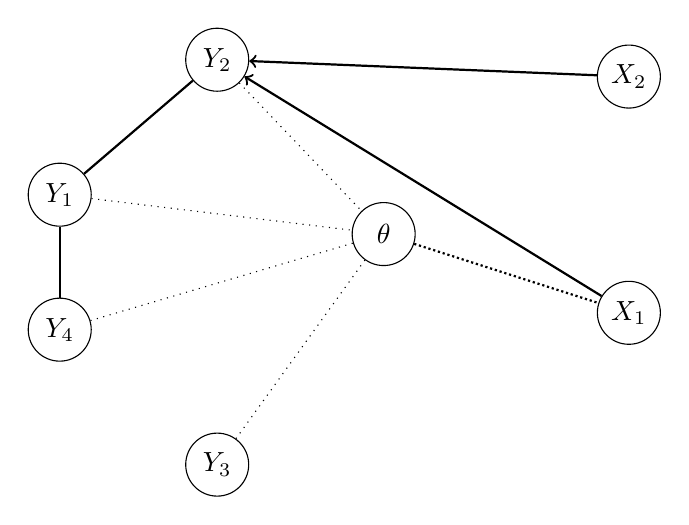
\begin{tikzpicture}[node distance=0.9cm and 2.3cm]
\node[nodecircle] (B) {$Y_2$};
\node[nodecircle,below=of B, xshift=-2cm] (A) {$Y_1$};
\node[nodecircle,below=of A] (D) {$Y_4$};
\node[nodecircle,below=of D, xshift=2cm] (C) {$Y_3$};

\node[nodecircle,right=of A, xshift=1cm,yshift=-0.5cm] (S) {$\theta$};

\node[nodecircle,right=of S,yshift=-1cm] (X) {$X_1$};
\node[nodecircle,right=of S,yshift=2cm] (Z) {$X_2$};

\draw[ld] (A)--(B);
\draw[ld] (A)--(D);

\draw[dotted] (A)--(S);
\draw[dotted] (B)--(S);
\draw[dotted] (C)--(S);
\draw[dotted] (D)--(S);

\draw[scoreedge] (S)--(X);

\draw[dif] (X)--(B);
\draw[dif] (Z)--(B);

\end{tikzpicture}
\end{center}
\end{example}
\end{mybox3}

for a grapchical Rasch model we use $\mathrm{SOURCE}(Y_i)$ to denote the set 
covariates $X_l$ where $D_{il}=1$ and $\mathrm{DIF}(X_l)$ to denote the set 
items $Y_l$ where $D_{il}=1$.

\section{Methods}\label{sec:it_sec}

This section describes the six-step item screening procedure. We assume that $V(\Theta)>0$. The analysis requires an association measure, a corresponding partial association measure, a method for calculating $p$-values, and a procedure for adjusting for multiple testing.

We use Goodman and Kruskal's $\gamma$ \citeyearpar{goodman-kruskal-1954} and partial $\gamma$ \citep{davis-1967}, as described in Appendix~\ref{sec:App-gamma}. The analyses use asymptotic $p$-values; Monte Carlo methods are an alternative \citep{north-2002}. We adjust for multiple testing using the Benjamini--Hochberg procedure \citeyearpar{benjamini-hochberg-1995}, described in Appendix~\ref{sec:App-multiple-testing}.

\subsection{Step 1: Analysis of consistency}

\subsubsection{M1} 

Test that there is a positive correlation between any pair of items. 

\subsubsection{M2} 

Test that any item $Y_a$ is positively related to its corresponding rest-score $R_a$, and all subscores $S_B$, where $Y_a\not\in B$.

\subsubsection{M3} 

Test that any exogenous variable $X_l$ that is positively related to $\Theta$ is also positively related to the total score $S$, to all subscores, $S_A$, and to all item responses $Y_i$.

\subsection{Step 2: Analysis of LD and DIF}\label{sec:ld-dif}

Use partial association coefficients to flag all item pairs exhibiting LD and all pairs of an item and a covariate that exhibit DIF. Test hypotheses of the form

\begin{align*}
    H_0^{DIF}: Y_i \bot X_j  \mid S \qquad \text{and} \qquad H_0^{LD}:Y_i \bot Y_{i'} \mid R_i,
\end{align*}

rejecting when the corresponding $p$-value is below $0.05$ after controlling for multiple testing.

\subsection{Step 3: Elimination of spurious evidence}

Step 3 filters out spurious evidence of LD and DIF through Steps 3(a), 3(b), and 3(c), described below.

\paragraph{Step 3(a): Elimination of spurious evidence of LD.} From the initial LD screening in Step 2, we look at all flagged evidence of LD and create five lists:

\coauthortodo{\textbf{Evidence lists.} Four lists are announced, but five are listed. The algorithm uses four active lists. Please reconcile these descriptions.\\ \textcolor{blue}{change made by STK: list "(v) item pairs with no significant partial $\gamma$ coefficients." removed, since no such list is created.}\\ \textcolor{orange}{change made by KACH: Fifth list is remainder.}}%

\begin{enumerate}
\item[(i)] pairs flagged with two significant positive partial $\gamma$ coefficients.
\item[(ii)] pairs flagged with two significant negative partial $\gamma$ coefficients.
\item[(iii)] pairs flagged with only one significant positive partial $\gamma$ coefficient.
\item[(iv)] pairs flagged with only one significant negative partial $\gamma$ coefficient. 
\item[(v)] All other item pairs. 
\end{enumerate}

For each pair, compute the weighted partial $\gamma$. Apply stepwise inclusion to the pairs flagged for LD, prioritizing pairs with two significant directional tests over those with only one. Within each priority group, select the pair with the largest absolute weighted partial $\gamma$ and retain it as genuine LD. Remove from further consideration all directional tests whose conditioning rest-score is defined by either item in the selected pair. Update the evidence lists (i)--(v) accordingly and repeat until no flagged pairs remain. 

\paragraph{Step 3(b): Elimination of spurious evidence for items with more than one
DIF source.} This procedure is implemented as Algorithm~\ref{alg:step3b} in Appendix~\ref{sec:AppAlgorithms}; no source is removed from the candidate list until all tests in the current iteration have been performed. Significance is assessed via the asymptotic $p$-value of the partial gamma test (Algorithm \ref{alg:part_gam} in Appendix~\ref{sec:AppAlgorithms}).

\paragraph{Step 3(c): Elimination of spurious evidence for sources with an apparent
DIF effect on more than one item.} This step applies the same elimination procedure as Step 3(b), but to the $DIF(X_i)$ lists rather than the $SOURCE(Y_i)$ lists, eliminating items exhibiting spurious DIF with respect to each exogenous variable; see Algorithm~\ref{alg:step3b} in Appendix~\ref{sec:AppAlgorithms}.

\paragraph{Combining Steps 3(b) and 3(c).} The two procedures run separately, and no final decision is made until both are complete. Their order therefore does not affect the combined decision. Each item--covariate pair carries two $p$-values, one from each step, and DIF is accepted as genuine only if both are significant.

\begin{mybox3}
\begin{example}\label{ex:step3b} \textbf{Step 3(b).}
Assume we have five items $\{Y_1,Y_2,Y_3,Y_4,Y_5\}$ and two exogenous variables
$\{X_1,X_2\}$. Suppose the initial DIF screening in Step 2 flags the following
item-covariate pairs:

\begin{table}[H]
\centering
\begin{tabular}{ccrr}
\hline
Item & Covariate & Partial $\gamma$ & $p$-value \\
\hline
$Y_1$ & $X_1$ & $0.42$ & $0.004$ \\
$Y_1$ & $X_2$ & $0.31$ & $0.030$ \\
$Y_3$ & $X_1$ & $-0.36$ & $0.018$ \\
$Y_5$ & $X_2$ & $0.55$ & $0.001$ \\
\hline
\end{tabular}
\caption{Initial evidence of DIF from Step 2.}
\label{tab:step3_example_initial}
\end{table}

From this $\mathrm{SOURCE}(Y_1)=\{X_1,X_2\}$, $\mathrm{SOURCE}(Y_3)=\{X_1\}$, $\mathrm{SOURCE}(Y_5)=\{X_2\}$, $\mathrm{DIF}(X_1)=\{Y_1,Y_3\}$, and $\mathrm{DIF}(X_2)=\{Y_1,Y_5\}$. Step 3(b) tests, for each item $Y_i$, whether each candidate source remains associated with $Y_i$ after conditioning on the score and the other candidate sources. Suppose it gives the following result:

\begin{table}[H]
\centering
\begin{tabular}{c c c c r l}
\hline
Iteration & Item & Candidate source & Hypothesis & $p$-value & 3(b) decision  \\
\hline
1 & $Y_1$ & $X_1$ & $Y_1 \perp X_1 \mid S, X_2$ & $0.060$ & Retain \\
  & $Y_1$ & $X_2$ & $Y_1 \perp X_2 \mid S,X_1$ & $0.210$ & Remove \\
  & $Y_3$ & $X_1$ & $Y_3 \perp X_1 \mid S$ & $0.018$ & Retain \\
  & $Y_5$ & $X_2$ & $Y_5 \perp X_2 \mid S$ & $0.001$ & Retain \\
2 & $Y_1$ & $X_1$ & $Y_1 \perp X_1 \mid S$ & $0.004$ & Retain \\
\hline
\end{tabular}
\caption{Hypothetical Step 3(b) elimination of spurious DIF sources}
\label{tab:step3_example_3b}
\end{table}
Thus Step 3(b) returns:
$\mathrm{SOURCE}^{(3b)}(Y_1)=\{X_1\}$, $\mathrm{SOURCE}^{(3b)}(Y_3)=\{X_1\}$, and
$\mathrm{SOURCE}^{(3b)}(Y_5)=\{X_2\}$.
\end{example}
\end{mybox3}

\begin{mybox3}
\begin{example}\label{ex:step3c} \textbf{Step 3(c).} 
Step 3(c) tests, for each covariate $X_l$, whether each candidate DIF item remains associated with $X_l$ after conditioning on the score and the other candidate items. Suppose this gives the following result:

\begin{table}[H]
\centering
\begin{tabular}{c c c c r l}
\hline
Iteration & Covariate & Candidate item & Hypothesis & $p$-value & 3(c) decision \\
\hline
1 & $X_1$ & $Y_1$ & $Y_1 \perp X_1 \mid S,Y_3$ & $0.090$ & Retain \\
  & $X_1$ & $Y_3$ & $Y_3 \perp X_1 \mid S,Y_1$ & $0.160$ & Remove \\
  & $X_2$ & $Y_5$ & $Y_5 \perp X_2 \mid S,Y_1$ & $0.200$ & Retain \\
  & $X_2$ & $Y_1$ & $Y_1 \perp X_2 \mid S,Y_5$ & $0.280$ & Remove \\
2 & $X_1$ & $Y_1$ & $Y_1 \perp X_1 \mid S$ & $0.004$ & Retain \\
  & $X_2$ & $Y_5$ & $Y_5 \perp X_2 \mid S$ & $0.001$ & Retain \\
\hline
\end{tabular}
\caption{Hypothetical Step 3(c) elimination of spurious DIF items.}
\label{tab:step3_example_3c}
\end{table}
Step 3(c) returns $\mathrm{DIF}^{(3c)}(X_1)=\{Y_1\}$ and $\mathrm{DIF}^{(3c)}(X_2)=\{Y_5\}$.

\end{example}
\end{mybox3}

\begin{mybox3}
\begin{example}\label{ex:step3b-and-c} \textbf{Combining 3(b) and 3(c).} An item-covariate pair is retained as genuine DIF only if it survives both procedures.

\begin{table}[H]
\centering
\begin{tabular}{c c c c c}
\hline
Item & Covariate & Survives Step 3(b) & Survives Step 3(c) & Conclusion \\
\hline
$Y_1$ & $X_1$ & Yes & Yes & Genuine DIF \\
$Y_1$ & $X_2$ & No & No & Spurious \\
$Y_3$ & $X_1$ & Yes & No & Spurious \\
$Y_5$ & $X_2$ & Yes & Yes & Genuine DIF \\
\hline
\end{tabular}
\caption{Combining Step 3(b) and Step 3(c).}
\label{tab:step3_example_combined}
\end{table}

Therefore, the final genuine DIF relations are
\[
Y_1 \sim X_1
\qquad \text{and} \qquad
Y_5 \sim X_2.
\]
Equivalently, the updated source and DIF sets are
\[
SOURCE(Y_1)=\{X_1\}, \qquad SOURCE(Y_5)=\{X_2\},
\]
and
\[
DIF(X_1)=\{Y_1\}, \qquad DIF(X_2)=\{Y_5\}.
\]
\end{example}
\end{mybox3}


\subsection{Step 4: Score--covariate associations}
We examine the structural association between the total score and exogenous variables via backward elimination: an exogenous covariate is retained as a structural predictor of the score if it remains conditionally associated with the score given the other retained covariates. This is outlined in Algorithm \ref{alg:step4} in Appendix~\ref{sec:AppAlgorithms}.

Retained covariates are treated as evidence of criterion validity and included in the initial graphical log-linear Rasch model (GLLRM); dropped covariates are judged to add no significant information about the score once the other candidates are controlled for, and are excluded.

\subsection{Step 5: Graph construction}

An initial graph is created by collecting outputs from steps 3 and 4. No new tests are performed. The graph records the nodes and the connections beyond the item--latent-trait edges. The IRT graph has the same nodes and edges, with measurement, score-association, and DIF edges directed and LD edges undirected. To construct the moralized marginal graph, we connect nodes that are parents of the same node, a process known as ``marrying parents''. We then replace the latent trait with a score node and add undirected score-to-item and item-to-item edges.


\subsection{Step 6: Tests of global Markov properties}
Before reporting an initial model, we retest the DIF and LD relations retained from Step 5 against the full structure, to check they are not artifacts of the simpler conditioning sets used earlier. For DIF, this is the test
\begin{align}
H_0^{C5}: Y_i \perp X_j
\mid
S,\ \operatorname{DIF}(X_j)\setminus\{Y_i\},\
\operatorname{SOURCE}(Y_i)\setminus\{X_j\}. \label{C5}
\end{align}
For each genuine LD pair $(Y_a,Y_b)$, we temporarily remove its edge and identify the remaining LD component containing each item. For each component, we form a subscore from the items outside it and identify the DIF sources associated with its member items. We then test the item pair in both directions, conditioning on the corresponding complementary subscore and DIF sources ($C7$ and $C9$; \citealp{kreiner-christensen-2011}). The edge is retained if at least one direction is significant.

\begin{mybox3}
\begin{example}
Assume we have a dataset with four items $Y_1,Y_2,Y_3,Y_4$ and two exogenous covariates $X_1,X_2$. Suppose within the dataset there exists DIF between the following pairs $(Y_2,X_1), (Y_3,X_1), (Y_2,X_2),$ LD between $(Y_1,Y_2), (Y_3,Y_4), (Y_1,Y_4)$, and finally $X_1$ is related to the score $S$. Step 6 now retests the DIF using \eqref{C5}.
\begin{table}[H]
\centering
\begin{tabular}{c c c c c}
\hline
Item & Candidate source & Hypothesis & $p$-value & Decision \\
\hline
$Y_2$ & $X_1$ & $Y_2 \perp X_1 \mid S, Y_3,X_2$ & $0.016$ & Retain\\
$Y_3$ & $X_1$ & $Y_3 \perp X_1 \mid S,Y_2$ & $0.210$ & Remove\\
$Y_2$ & $X_2$ & $Y_2 \perp X_2 \mid S,X_1$ & $0.04$ & Retain \\
\hline
\end{tabular}
\caption{Hypothetical tests to determine if DIF edges should be retained.}
\label{tab:step6_dif_example}
\end{table}
Next we check whether the LD edges should be retained: take the pair $(Y_1,Y_2)$, cut their edge, and consider the LD connections still available from each item.
% Temporary removal of LD edge (Y_1,Y_2)
\begin{center}
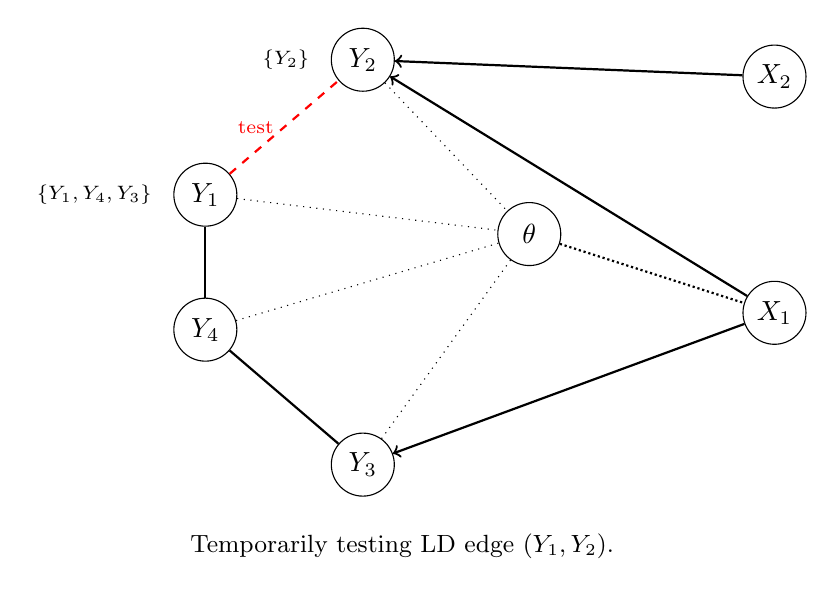
\begin{tikzpicture}[node distance=0.9cm and 2.3cm]
\node[nodecircle] (B) {$Y_2$};
\node[nodecircle,below=of B, xshift=-2cm] (A) {$Y_1$};
\node[nodecircle,below=of A] (D) {$Y_4$};
\node[nodecircle,below=of D, xshift=2cm] (C) {$Y_3$};

\node[nodecircle,right=of A, xshift=1cm,yshift=-0.5cm] (S) {$\theta$};

\node[nodecircle,right=of S,yshift=-1cm] (X) {$X_1$};
\node[nodecircle,right=of S,yshift=2cm] (Z) {$X_2$};

\draw[removed] (A)--node[left]{\scriptsize test} (B);
\draw[ld] (C)--(D);
\draw[ld] (A)--(D);

\draw[dotted] (A)--(S);
\draw[dotted] (B)--(S);
\draw[dotted] (C)--(S);
\draw[dotted] (D)--(S);
% should the next three be here when we are using theta instead of S?
% \draw[dotted] (B)--(C);
% \draw[dotted] (B)--(D);
% \draw[dotted] (A)--(C);

\draw[scoreedge] (S)--(X);

\draw[dif] (X)--(B);
\draw[dif] (X)--(C);
\draw[dif] (Z)--(B);

\node[left=0.15cm of A] {\scriptsize $\{Y_1,Y_4,Y_3\}$};
\node[left=0.15cm of B] {\scriptsize $\{Y_2\}$};

\node[below=0.35cm of C,xshift=.5cm]
{\small Temporarily testing LD edge $(Y_1,Y_2)$.};
\end{tikzpicture}
\end{center}

%\coauthortodo{\textbf{Set notation.} Earlier, $DIF(X)$ denotes items. Here, $DIF(C_A)$ and $DIF(C_B)$ mean covariate sources. Please define the notation for sources associated with item sets.\\ \textcolor{blue}{notation fixed by STK; it should ofc be "$\text{SOURCE}(C_A)$" and "$\text{SOURCE}(C_B)$"}}%

The graph shows that the remaining LD components are
\begin{equation}
    C_{Y_1}=\{Y_1,Y_4,Y_3\},\qquad C_{Y_2}=\{Y_2\}.
\end{equation}
The complements of $C_{Y_1}$ and $C_{Y_2}$ are taken within the full item set. Summing the responses to the items in each complement gives the subscores $S_{C_{Y_1}^c}$ and $S_{C_{Y_2}^c}$. Each test also conditions on the DIF sources associated with the items in the corresponding LD component: $X_1$ for $C_{Y_1}$, and $X_1$ and $X_2$ for $C_{Y_2}$. The two hypotheses are
\begin{align*}
    C7:\ Y_1\bot Y_2\mid S_{C_{Y_1}^c},\text{SOURCE}(C_{Y_1}) \quad = \quad Y_1\bot Y_2\mid S_{C_{Y_1}^c},X_1,
\end{align*}
and
\begin{equation*}
    C9:\ Y_1\bot Y_2\mid S_{C_{Y_2}^c},\text{SOURCE}(C_{Y_2}) \quad = \quad Y_1\bot Y_2\mid S_{C_{Y_2}^c},X_2,X_1.
\end{equation*}
Doing this for all LD edges, suppose we observe the following table of tests

% \coauthortodo{\textbf{Degenerate tests.} Removing A--B gives $S_{C_A^c}=B$; removing C--D gives $S_{C_D^c}=C$. These tests condition on a tested item, so partial $\gamma$ is undefined. Please check $p=0.016$ and $0.03$. \\ \textcolor{blue}{Changes accepted an implemented by STK, cf the reason given in mail sent 13/09}}%

\begin{table}[H]
\centering
\begin{tabular}{c c c c}
\hline
LD pair & Hypothesis & $p$-value & Decision \\
\hline
$(Y_1,Y_2)$ & $Y_2 \bot Y_1 \mid S_{C_{Y_1}^c},X_1$ & NA & not supported/undefined \\
$(Y_1,Y_2)$ & $Y_2 \perp Y_1 \mid S_{C_{Y_2}^c},X_1,X_2$ & $0.510$ & not supported\\
$(Y_3,Y_4)$ & $Y_3 \perp Y_4 \mid S_{C_{Y_3}^c},X_1$ & $0.02$ & supported \\
$(Y_3,Y_4)$ & $Y_3 \perp Y_4 \mid S_{C_{Y_4}^c},X_1,X_2$ & NA & not supported/undefined \\
$(Y_1,Y_4)$ & $Y_1 \perp Y_4 \mid S_{C_{Y_1}^c},X_1,X_2$ & $0.2$ & not supported \\
$(Y_1,Y_4)$ & $Y_1 \perp Y_4 \mid S_{C_{Y_4}^c},X_1$ & $0.33$ & not supported \\
\hline  
\end{tabular}
\caption{Hypothetical tests to determine if LD edges should be retained.}
\label{tab:step6_ld_example}
\end{table}

% \coauthortodo{\textbf{Step 6.} Please check the paragraph and final graph against the table. The stated rule and $p$-values imply keeping $(A,B)$ and $(C,D)$, and removing $(A,D)$. The paragraph and graph reverse the latter two decisions.\\ \textcolor{blue}{Changes made by STK: updated graph to be in accordance with the stated rule and p-values from the hypothetical table 6}}% Since an LD edge is removed if and only if the pair fails to achieve a significant $p$-value for both Step 6 LD tests, we conclude the two LD edges $(Y_1,Y_2)$ and $(Y_1,Y_4)$ should be dropped, while the edge between $(Y_3,Y_4)$ is kept. Thus, we are left with the final Step 6 graph below.

\begin{center}
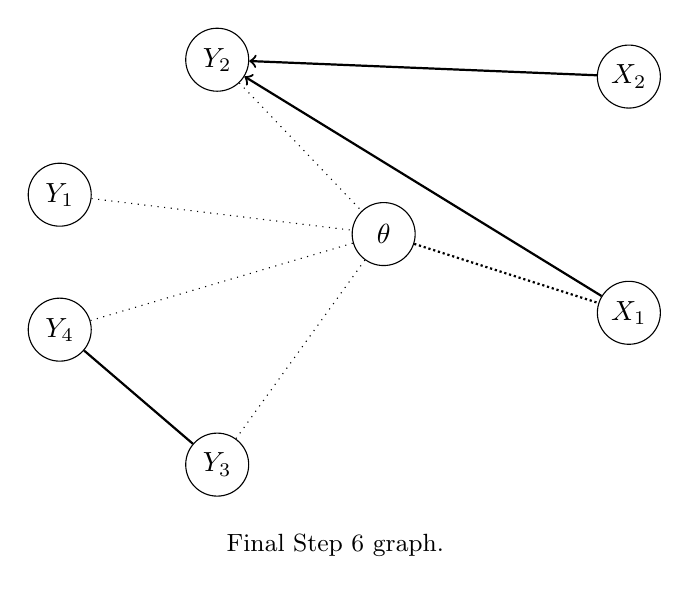
\begin{tikzpicture}[node distance=0.9cm and 2.3cm]
\node[nodecircle] (B) {$Y_2$};
\node[nodecircle,below=of B, xshift=-2cm] (A) {$Y_1$};
\node[nodecircle,below=of A] (D) {$Y_4$};
\node[nodecircle,below=of D, xshift=2cm] (C) {$Y_3$};

\node[nodecircle,right=of A, xshift=1cm,yshift=-0.5cm] (S) {$\theta$};

\node[nodecircle,right=of S,yshift=-1cm] (X) {$X_1$};
\node[nodecircle,right=of S,yshift=2cm] (Z) {$X_2$};

%\draw[ld] (A)--(B);
\draw[ld] (C)--(D);

\draw[dotted] (A)--(S);
\draw[dotted] (B)--(S);
\draw[dotted] (C)--(S);
\draw[dotted] (D)--(S);
% Should the next three be there when we are using theta instead of S?
% \draw[dotted] (B)--(C);
% \draw[dotted] (D)--(B);
% \draw[dotted] (A)--(C);

\draw[scoreedge] (S)--(X);

\draw[dif] (X)--(B);
\draw[dif] (Z)--(B);

\node[below=0.35cm of C,xshift=1.5cm]
{\small Final Step 6 graph.};
\end{tikzpicture}
\end{center}
    \end{example}
\end{mybox3}



\section{Results}

We apply the screening procedure to data from $99$ respondents who completed the $10$-item Actinic Keratosis Quality of Life (AKQoL) questionnaire ($Q1$--$Q10$, each scored $0$--$3$). Two covariates were also recorded: sex (\texttt{woman}, $1=$ woman) and age (\texttt{Alder}, in years). All $99$ respondents have complete item and covariate data.

\subsection{Step 1}
All items pass M2: each is positively associated with its rest-score, with the smallest association observed for $Q9$ ($\gamma=0.078$). Both M1 and M3 flag $Q9$. M1 fails because the association between $Q5$ and $Q9$ is negative ($\gamma=-0.168$); all other $\binom{10}{2}-1$ item pairs have non-negative associations. For M3, age passes because its associations with the score and all items are consistently negative (score $\gamma=-0.164$). Sex fails because its association with $Q9$ ($\gamma=-0.121$) has the opposite sign to its association with the score ($\gamma=0.338$). Its associations with all other items have the same sign as its association with the score. Because the inconsistencies in M1 and M3 are confined to $Q9$, we proceed to Step 2.

\subsection{Step 2}
Controlling the false discovery rate (FDR) with Benjamini--Hochberg, the initial screen flags two DIF relations and four candidate LD pairs.

% \coauthortodo{\textbf{DIF threshold.} Q4--Alder has $p_{\mathrm{adj}}=0.062>0.05$, yet is counted and carried forward as an initial DIF candidate. Please reconcile the BH adjustment family, decision threshold, and table with the stated 5\% criterion. \\ \textcolor{blue}{The output of twigg::screen\_DIF() contains 3 p-value columns. Raw, iarm::partgam\_DIF's adjusted p-value and "your.adjusted.p" which twigg computes itself. The one reported here "$p_{adj}$" is iarm::partgam\_DIF's adjusted p-value, which computes it without ranking the p-values. However twigg takes all the raw p-values, ranks them and then computes the adjusted p-value. So the p-value included here should probably be the "your.adjusted.p" since this is the p-value twigg uses to determine significance. - i have changed the p-values in the from the "padj.BH" values to the "your.adjusted.p" values, and the "." to a "*" for Q4-Alder}}%

\begin{table}[H]
\centering
\begin{tabular}{@{}llcccc@{}}
\toprule
Item & Source & partial $\gamma$ & $p$ & $p_{\mathrm{adj}}$ & sig. \\
\midrule
$Q4$ & Alder & $0.383$ & $0.0031$ & $0.031$ & * \\
$Q5$ & woman & $0.727$ & $0.0008$ & $0.017$ & * \\
\bottomrule
\end{tabular}
\caption{Initial evidence of DIF (Step 2).}
\label{tab:ak_step2_dif}
\end{table}
\begin{table}[H]
\centering
\begin{tabular}{@{}llcccc@{}}
\toprule
Item 1 & Item 2 & partial $\gamma$ & $p$ & $p_{\mathrm{adj}}$ & sig. \\
\midrule
$Q5$  & $Q6$  & $0.650$  & $0.0005$ & $0.046$ & * \\
$Q3$  & $Q9$  & $-0.588$ & $0.0003$ & $0.026$ & * \\
$Q6$  & $Q9$  & $-0.629$ & $0.0004$ & $0.036$ & * \\
$Q3$  & $Q10$ & $-0.755$ & $<0.0001$ & $<0.0001$ & *** \\
\bottomrule
\end{tabular}
\caption{Initial evidence of LD (Step 2), flagged in at least one conditioning direction.}
\label{tab:ak_step2_ld}
\end{table}

\subsection{Step 3}
\subsubsection{Step 3(a)}
The stepwise inclusion algorithm accepts $(Q3,Q10)$ (weighted partial $\gamma=-0.694$) and $(Q5,Q6)$ (weighted partial $\gamma=0.494$) as genuine LD. The remaining candidates, $(Q3,Q9)$ and $(Q6,Q9)$, are disregarded as spurious once $Q3$ and $Q6$ are used to define the rest-scores for the accepted pairs -- consistent with $Q9$'s already anomalous behavior in Step 1.
\begin{table}[H]
\centering
\begin{tabular}{@{}llc@{}}
\toprule
Item 1 & Item 2 & weighted partial $\gamma$ \\
\midrule
$Q3$ & $Q10$ & $-0.694$ \\
$Q5$ & $Q6$  & $0.494$ \\
\bottomrule
\end{tabular}
\caption{Genuine LD pairs after the Step 3(a) inclusion algorithm.}
\label{tab:ak_step3a}
\end{table}

\subsubsection{Steps 3(b) and 3(c)}
Each flagged item has exactly one candidate DIF source and each source only one candidate item, so the elimination algorithms of Steps 3(b) and 3(c) have nothing to condition away: both relations from Step 2 pass through unchanged and are carried forward as candidate genuine DIF.
\begin{table}[H]
\centering
\begin{tabular}{@{}llccc@{}}
\toprule
Item & Source & partial $\gamma$ & $p$ & Conclusion \\
\midrule
$Q4$ & Alder & $0.383$ & $0.0031$ & DIF \\
$Q5$ & woman & $0.727$ & $0.0008$ & DIF \\
\bottomrule
\end{tabular}
\caption{Result of combining Steps 3(b) and 3(c) (asymptotic $p$-values, both conditioning sets are $S$).}
\label{tab:ak_step3bc}
\end{table}

\subsection{Step 4}
Backward elimination retains \texttt{woman} and drops \texttt{Alder} as a structural predictor of the score.
\begin{table}[H]
\centering
\begin{tabular}{@{}lcccl@{}}
\toprule
Covariate & partial $\gamma$ & $p$ & $\mathcal{C}$ & S.C.V. \\
\midrule
woman & $0.357$ & $0.017$ & Alder & TRUE \\
Alder & $-0.054$ & $0.693$ & woman & FALSE \\
\midrule
woman (final) & $0.338$ & $0.008$ & None & TRUE \\
\bottomrule
\end{tabular}
\caption{Step 4 backward elimination search. $\mathcal{C}$ is the conditioning set; S.C.V.\ abbreviates ``supports criterion validity''.}
\label{tab:ak_step4}
\end{table}

\subsection{Step 5}
Collecting the Step 3 and Step 4 results gives the tentative GLLRM: a measurement edge $\theta\to Q_i$ for each item, a score association \texttt{woman}$\,\to\theta$, DIF edges Alder$\,\to Q4$ and woman$\,\to Q5$, and LD edges $(Q3,Q10)$ and $(Q5,Q6)$. Because \texttt{Alder} was dropped in Step 4, it enters the graph only through its DIF edge on $Q4$ and has no direct association with $\theta$.
\begin{table}[H]
\centering
\begin{tabular}{@{}lll@{}}
\toprule
From & To & Edge type \\
\midrule
$\theta$ & $Q1,\dots,Q10$ & measurement \\
woman & $\theta$ & score association \\
Alder & $Q4$ & DIF \\
woman & $Q5$ & DIF \\
$Q3$ & $Q10$ & local dependence \\
$Q5$ & $Q6$ & local dependence \\
\bottomrule
\end{tabular}
\caption{Step 5 IRT graph edges (\texttt{build\_gllrm\_graph} / \texttt{build\_irt\_graph}).}
\label{tab:ak_step5}
\end{table}

\subsection{Step 6}

% \coauthortodo{\textbf{Repeated DIF tests.} With one item per source and one source per item, $C5$ again conditions only on $S$. Why do the same $\gamma$s now have $p=0.051,0.032$ rather than $0.0031,0.0008$? Please state any change in data, test, or adjustment.\\ \textcolor{blue}{p-values changed by STK, cf explanation in email sent 13/9. Feel free to re-run the code yourself with the updated step6\_check\_gllrm function in twigg (I have already done so and it produces the correct p-values when p\_value\_method is set to "asymptotic".}}%

The retained DIF and LD edges are retested under the conditioning sets implied by the Step 5 graph. For DIF this is the $C5$ hypothesis of \eqref{C5}; for each LD pair the two $C7$/$C9$ hypotheses are tested, with an edge kept if at least one is significant.

\begin{table}[H]
\centering
\begin{tabular}{@{}llccl@{}}
\toprule
Edge & Hypothesis & partial $\gamma$ & $p$ & Decision \\
\midrule
Alder $\to Q4$ & $C5$ & $0.383$ & $0.0031$ & Retained \\
woman $\to Q5$ & $C5$ & $0.727$ & $0.0008$ & Retained \\
\bottomrule
\end{tabular}
\caption{Step 6 retesting of the Step 5 DIF edges (\texttt{step6\_check\_gllrm}).}
\label{tab:ak_step6_dif}
\end{table}

% \coauthortodo{\textbf{(STK) monte carlo p-values}. These p-values are produced via the monte carlo method since i just now implemented the opportunity to change it.. Should they be changed for consistency and reproducibility purposes?}

\begin{table}[H]
\centering
\begin{tabular}{@{}lccccl@{}}
\toprule
Edge & $C7$: $\gamma$ & $C7$: $p$ & $C9$: $\gamma$ & $C9$: $p$ & Decision \\
\midrule
$Q3$--$Q10$ & $-0.611$ & $0.0019$ & $-0.755$ & $<0.0001$ & Retained \\
$Q5$--$Q6$  & $0.765$  & $0.0002$  & $0.362$  & $0.142$  & Retained \\
\bottomrule
\end{tabular}
\caption{Step 6 retesting of the Step 5 LD edges. An edge is retained if at least one of $C7$/$C9$ is significant.}
\label{tab:ak_step6_ld}
\end{table}
The DIF edge Alder$\,\to Q4$ fails its $C5$ test ($p=0.051$) and is removed, along with the moralized-graph edge it implied; woman$\,\to Q5$ is retained. Both LD pairs survive, each with at least one significant conditioning direction. The final GLLRM for the AK data therefore retains all $10$ items, one genuine DIF effect (woman on $Q5$), two genuine LD pairs ($Q3$--$Q10$ and $Q5$--$Q6$), and one score-covariate association (woman); despite an initial signal in Steps 1--3, \texttt{Alder} shows no surviving effect once the full screening procedure is applied.


\section{Discussion}
\coauthortodo{\textbf{Subscore count.} Excluding the empty subset would give $2^{k-1}-1$. Please check the count in this paragraph.\\
\textcolor{blue}{Change accepted and implemented by STK. Andreas' comment is correct.}}%
The implementation of M2 checks associations between items and their corresponding rest-scores. M3 examines associations between covariates and the total score and checks their direction against the item--covariate associations. These screening checks do not exhaustively evaluate all possible subscores. This keeps the procedure computationally feasible because the number of candidate subscores grows exponentially with the number of items. For $k$ items, the number of subscores excluding the item under examination and the zero subscore is $2^{k-1}-1$.

In Step 3(a), the inclusion algorithm prioritizes pairs with two significant directional LD tests over pairs with only one. Within each group, pairs are ranked by the absolute value of the weighted partial gamma coefficient, allowing both positive and negative associations to be selected. This ordering defines the algorithm's screening priorities. As directional tests are removed from consideration, a pair can move from the group with two significant tests to the group with one. The weighted coefficient accounts for the number of comparable pairs contributing to each directional estimate, rather than assigning equal weight to both estimates through an arithmetic mean.

A negative partial gamma indicates that higher scores on one item tend to be associated with lower scores on the other, conditional on the variables used in the test. One possible explanation is that the items assess different methods or dimensions \citep{kreiner-christensen-2004}. Such a pattern warrants consideration of whether the questionnaire should be analyzed as a single scale or as separate subscales.


Two decisions are central to DIF screening. First, Steps 3(b) and 3(c) are complementary: a final decision is made only after both procedures have been completed and their results compared. A DIF edge is retained only if it survives both steps. This conservative rule reduces the risk of retaining spurious DIF, at the cost of potentially removing weaker genuine relationships. The procedure starts with a broad set of candidate LD and DIF relations in Step 2 and progressively reduces that set, with retained edges tested again in Step 6. Second, the calculation of $p$-values requires a choice of method. We use asymptotic $p$-values throughout. These are fast to compute but may be less reliable when contingency tables are sparse and the conditioning strata contain few observations.

Steps 5 and 6 report graph structures without drawing them. They return the nodes, edges, edge types, and directions, leaving visualization to the user. Step 5 constructs an evidence graph from the retained LD, DIF, and score--covariate associations. This graph summarizes the screening results and should not be interpreted as a fully validated model. Step 6 retests the retained edges using the conditioning sets implied by the graph.

\newpage
\bibliography{reference}

\newpage
\begin{appendices}
\section{}\label{sec:AppGeneral}
\section*{The General Ordinal Item Response Model}

For ease of exposition, the main text restricts attention to dichotomous items, $Y_i\in\{0,1\}$. Here we give the corresponding formulas for the general case of ordinal items with $M+1$ response categories, $Y_i\in\{0,1,\ldots,M\}$ (assuming, for ease of notation, that all items have the same number of response categories).

The parametric form of the response probabilities is
$$
P(Y_i=y|\theta)=\frac{\exp(y\theta+\alpha_{iy})}{\sum_{z=0}^M\exp(z\theta+\alpha_{iz})},
$$
which reduces to the dichotomous form used in the main text when $M=1$ and $\alpha_{i0}=0$, $\alpha_{i1}=\alpha_i$.

Combining requirements (ii)-(iv) of Section~\ref{sec:models_measurement}, the Rasch model in vector form is
\begin{align}
P(\boldsymbol{Y} = \boldsymbol{y} | \boldsymbol{X} = \boldsymbol{x}, \theta) =\exp\left(\alpha_0+\theta S+\sum_{i=1}^k\alpha_{iy_i}\right)
\end{align}
where
$$
\alpha_0=-\log\left(\prod_{i=1}^k\sum_{z=0}^M\exp(z\theta+\alpha_{iz})\right)
$$
is a normalizing constant that does not depend on the observed data $(\boldsymbol{y},\boldsymbol{x})$. Note that this reduces to the dichotomous normalizing constant of the main text when $M=1$ and that it $S$ is also sufficient in this general model.

The formula above specifies a log-linear model containing only main effects, and this model is easily extended to include (i) interaction terms between item pairs (to model LD) and (ii) interaction terms between item and exogenous variable pairs (to model DIF). This leads to the following form for the graphical Rasch model for polytomous items 
\begin{align}
P(\mathbf{Y}=\mathbf{y}\mid \Theta=\theta,\mathbf{X}=\mathbf{x}) = \exp\Big(\alpha_0+\theta S+\sum_{i=1}^k\alpha_i+(\star)\Big),
\end{align}
where
\begin{align}
(\star)=\sum_{i=1}^{n_L}\lambda_i(u_i,v_i)+ \sum_{i=1}^{n_D}\delta_i(a_i,z_i)+\sum_{i=1}^{n_G}\mu_i(g_i).
\end{align}
Here $n_D$ denotes the total number of DIF pairs $D=(D_1,\dots,D_{n_D})$ with $D_i=(A_i,Z_i)$, where $A_i\in\{Y_1,\dots,Y_k\}$, and $Z_i\in\{X_1,\dots,X_m\}$ is a source of DIF for $A_i$. $n_L$ denotes the total set of LD pairs with $L=(L_1,\dots,L_{n_L})$ with $L_i=(U_i,V_i)\subset \{Y_1,\dots,Y_k\}$. Lastly, $n_G$ is the total set of interactions with more complex DIF or LD structure, $G=(G_1,\dots,G_{n_G})$ with $G_i\subset \{Y_1,\dots,Y_k,X_1,\dots,X_m\}$ \cite{kreiner-christensen-2011}. 

Note that $S$ is also sufficient for $\theta$ in this model.
\end{appendices}

\begin{appendices}

\section{Association measures}\label{sec:App-gamma}
%\begin{breakablealgorithm}
\caption{Elimination of Spurious DIF Items for One Exogenous Covariate $X_j$}
\label{alg:step3c}

\begin{algorithmic}[1]
\Require Dataset with item responses and exogenous covariates; exogenous covariate $X_j$; item set $\mathcal{I}$; initial DIF set for $X_j$, $\mathrm{DIF}(X_j)$; and significance level $\alpha$

\Ensure Final set of items exhibiting genuine DIF with respect to $X_j$; $\widehat{\mathrm{DIF}}(X_j)$.

\State Compute the total score
\[
S = \sum_{Y_k \in \mathcal{I}} Y_k .
\]

\State Initialize
\[
\mathcal{S}_j^{(0)} \gets \mathrm{DIF}(X_j).
\]

\State Set $t \gets 0$.

\Repeat

    \State Let
    \[
    \mathcal{P}_j^{(t)} \gets \mathcal{S}_j^{(t)}
    \]
    denote the DIF set used during the current pass.

    \State Set
    \[
    Y_{\mathrm{drop}} \gets \emptyset,
    \qquad
    p_{\mathrm{drop}} \gets -\infty .
    \]

    \ForAll{$Y_i \in \mathcal{P}_j^{(t)}$}

        \State Use Algorithm~\ref{alg:mc_cond_independence} to test
        \[
        H_0:
        Y_i \perp X_j
        \mid
        S,\,
        \mathcal{P}_j^{(t)} \setminus \{Y_i\}.
        \]

        \State Let $p_i^{(t)}$ denote the corresponding $p$-value.

        \If{$p_i^{(t)} > \alpha$ and $p_i^{(t)} > p_{\mathrm{drop}}$}
            \State Set
            \[
            Y_{\mathrm{drop}} \gets Y_i,
            \qquad
            p_{\mathrm{drop}} \gets p_i^{(t)} .
            \]
        \EndIf

    \EndFor

    \If{$Y_{\mathrm{drop}} = \emptyset$}
        \State Stop the elimination procedure.
    \Else
        \State Remove the non-significant item with the highest $p$-value found in the current pass:
        \[
        \mathcal{S}_j^{(t+1)}
        \gets
        \mathcal{S}_j^{(t)}
        \setminus
        \{Y_{\mathrm{drop}}\}.
        \]

        \State Set $t \gets t+1$.
    \EndIf

\Until{no item is removed or $\mathcal{S}_j^{(t)} = \emptyset$}

\State Set
\[
\widehat{\mathrm{DIF}}(X_j)
\gets
\mathcal{S}_j^{(t)} .
\]

\State \Return $\widehat{\mathrm{DIF}}(X_j)$

\end{algorithmic}
\end{breakablealgorithm}
Goodman and Kruskal's $\gamma$ \citeyearpar{goodman-kruskal-1954} measures association between two ordinal variables. It compares the numbers of concordant pairs of observations, $C$, and discordant pairs, $D$. A concordant pair has the same ordering on both variables; a discordant pair has opposite orderings. The coefficient is

\begin{equation}
\gamma^{GK} = \frac{C-D}{C+D}.
\end{equation}

Partial $\gamma$ \citep{davis-1967} measures association within strata defined by the conditioning variables. For example, testing DIF between $Y_i$ and $X_j$ requires conditioning on the total score $S$. We therefore stratify the data by the observed values of $S$ and count concordant and discordant pairs within each stratum. Let $n$ denote the number of strata, indexed by $l=1,\dots,n$ to keep the stratum index distinct from the item indices $i,j$. Pooling the counts across strata gives the partial gamma coefficient, which can also be expressed as a weighted sum of the stratum-specific gamma coefficients:
\begin{align}
    \hat{\gamma}_{Y_i\bot X_j\mid S} &= \sum_{l=1}^n w_l\gamma^{GK}_l = \sum_{l=1}^n\frac{(C_l+D_l)}{\sum_{l=1}^n(C_l+D_l)}\frac{C_l-D_l}{C_l+D_l} \\
    &= \frac{\sum_{l=1}^n(C_l-D_l)}{\sum_{l=1}^n(C_l+D_l)} = \frac{\sum_{l=1}^nC_l-\sum_{l=1}^nD_l}{\sum_{l=1}^nC_l+\sum_{l=1}^nD_l}.
\end{align}
Each stratum's weight is its number of comparable pairs (concordant plus discordant) divided by the total number of comparable pairs across all strata. Strata with more comparable pairs therefore contribute more to the pooled coefficient \citep{agresti-1984}. If a stratum $l$ has no comparable pairs, $C_l+D_l=0$, its stratum-specific coefficient $\gamma^{GK}_l$ is undefined and the weighted-sum expression contains the indeterminate term $0\cdot(0/0)$. We adopt the convention that such a stratum contributes nothing to either sum, i.e., it is simply omitted from the stratification: since $C_l=D_l=0$ leaves both $\sum_l C_l$ and $\sum_l D_l$ unchanged, this is exactly what the pooled-count form on the right already does, and it matches how Algorithm~\ref{alg:part_gam} in Appendix~\ref{sec:AppAlgorithms} is computed, which skips any stratum whose contingency table has fewer than two rows or columns.

Both coefficients compare the difference between concordant and discordant pair counts with their sum. When defined, they lie in $[-1,1]$: values closer to $1$ indicate stronger positive association, and values closer to $-1$ indicate stronger negative association \citep{agresti-1984}. If there are no comparable pairs, the denominator is zero and the coefficient is undefined.

\end{appendices}

\begin{appendices}
\section{}\label{sec:App-multiple-testing}
\subsection{The Multiple Testing Problem}
Step 2 involves multiple hypothesis tests (Section~\ref{sec:ld-dif}). We account for multiple testing by controlling the false discovery rate (FDR).

\subsubsection{The Benjamini--Hochberg Procedure}
\coauthortodo{\textbf{Ordered p-values.} Please check whether the ordering should use $\leq$ to allow ties.\\
\textcolor{blue}{Cange accepted and implemented by STK. tiwgg uses "stats::p.adjust(..., method = "BH")" which handles ties trhough R's standard implementation, thus allowing for ties. So the inequalities should be weak and not hard.}}%
We use the Benjamini--Hochberg procedure to control the FDR \citep{benjamini-hochberg-1995}. For $T$ tests, rank the raw $p$-values in ascending order, $p_1\leq p_2\leq \dots \leq p_T$. At the chosen FDR level $\alpha$, find the largest $t$ such that $p_t\leq \frac{t}{T}\alpha$ and reject the null hypotheses corresponding to $p_i$, $i=1,\dots,t$. If no $p$-value meets this condition, no null hypotheses are rejected. The same decisions can be obtained by comparing the Benjamini--Hochberg-adjusted $p$-values with $\alpha$.

\end{appendices}

\begin{appendices}
\section{}\label{sec:AppAlgorithms}
\section*{Algorithms}

This appendix collects the pseudocode for the algorithms implementing the item screening procedure described in Section~\ref{sec:it_sec}, in the order in which they are used.

\subsection*{Step 2: Partial Gamma Coefficient}
$A$ and $B$ are variables that correspond to distinct items if we check for LD. If we check for DIF, one is an item and one is an exogenous variable. All rejected tests are flagged and we move onto the next step.

\begin{breakablealgorithm}
\caption{Partial $\gamma$ coefficient for testing $A \bot B \mid \mathcal{C}$}
\label{alg:part_gam}

\begin{algorithmic}
\Require Dataset with item responses and exogenous covariates; variables $A$ and $B$; conditioning variables $\mathcal{C}$
\Ensure Partial gamma coefficient $\gamma_{A \bot B \mid \mathcal{C}}$

\State Initialize
\[
C \gets 0,
\qquad
D \gets 0.
\]

\State Stratify the dataset according to the joint levels of the conditioning variable(s) $\mathcal{C}$.
\State Let $n$ denote the number of resulting strata.

\For{$l = 1,\ldots,n$}

    \State Let $\mathcal{D}_l$ denote the observations in stratum $l$.

    \If{$\mathcal{D}_l$ contains fewer than two observations}
        \State Skip stratum $l$.
    \EndIf

    \State Construct the contingency table of $A$ and $B$ within stratum $l$.

    \If{the contingency table has fewer than two rows or fewer than two columns}
        \State Skip stratum $l$.
    \EndIf

    \State Compute the number of concordant pairs in stratum $l$:
    \[
    C_l \gets \#\{\text{concordant pairs in stratum } l\}.
    \]

    \State Compute the number of discordant pairs in stratum $l$:
    \[
    D_l \gets \#\{\text{discordant pairs in stratum } l\}.
    \]

    \State Update
    \[
    C \gets C + C_l,
    \qquad
    D \gets D + D_l.
    \]

\EndFor

\If{$C + D = 0$}
    \State \Return $\mathrm{NA}$
\EndIf

\State Compute
\[
\gamma_{A \bot B \mid \mathcal{C}}
\gets
\frac{C-D}{C+D}.
\]

\State \Return $\gamma_{A \bot B \mid \mathcal{C}}$

\end{algorithmic}
\end{breakablealgorithm}

\subsection*{Step 3(a): Elimination of Spurious Local Dependence}
\begin{breakablealgorithm}
\caption{Elimination of Spurious Local Dependence}
\label{alg:LD_eli_algo}

\begin{algorithmic}[1]
\Require Set of significant local dependence hypotheses from the initial LD screening.
For each item pair $\{Y_i,Y_{i'}\}$, at most two directional hypotheses can be significant:
\[
H_{ii'}^{(i)}:\; Y_i \perp Y_{i'} \mid R_i,
\qquad
H_{ii'}^{(i')}:\; Y_i \perp Y_{i'} \mid R_{i'}.
\]
Let $\gamma_{ii'}^{(i)}$ and $\gamma_{ii'}^{(i')}$ denote the corresponding partial
$\gamma$ coefficients, and let $w_{ii'}^{(i)}$ and $w_{ii'}^{(i')}$ denote the
corresponding numbers of comparable pairs.

\Ensure Reduced set $\mathcal{G}$ of item pairs considered to exhibit genuine local dependence.

\State Initialize the set of active significant directional LD hypotheses:
\[
\mathcal{H}
\gets
\left\{
H_{ii'}^{(k)}
:
H_{ii'}^{(k)} \text{ is significant},
\;
k \in \{i,i'\}
\right\}.
\]

\State Initialize the set of genuine LD relations:
\[
\mathcal{G} \gets \emptyset.
\]

\State For each item pair $\{Y_i,Y_{i'}\}$ represented in the initial LD
screening, compute the pair-level weighted partial gamma
\[
WPG_{ii'}
=
\frac{
w_{ii'}^{(i)}\gamma_{ii'}^{(i)}
+
w_{ii'}^{(i')}\gamma_{ii'}^{(i')}
}{
w_{ii'}^{(i)} + w_{ii'}^{(i')}
}.
\]

\While{$\mathcal{H} \neq \emptyset$}

    \State Identify all unordered item pairs $\{Y_i,Y_{i'}\}$ represented by at least one
    hypothesis in the current active set $\mathcal{H}$.

    \State Using only the currently active significant directional hypothesis, partition
    the represented item pairs into four evidence lists:
    \[
    \mathcal{L}_{++}^{(2)}
    =
    \left\{
    \{Y_i,Y_{i'}\}
    :
    H_{ii'}^{(i)} \in \mathcal{H},\;
    H_{ii'}^{(i')} \in \mathcal{H},\;
    \gamma_{ii'}^{(i)} > 0,\;
    \gamma_{ii'}^{(i')} > 0
    \right\},
    \]
    \[
    \mathcal{L}_{--}^{(2)}
    =
    \left\{
    \{Y_i,Y_{i'}\}
    :
    H_{ii'}^{(i)} \in \mathcal{H},\;
    H_{ii'}^{(i')} \in \mathcal{H},\;
    \gamma_{ii'}^{(i)} < 0,\;
    \gamma_{ii'}^{(i')} < 0
    \right\},
    \]
    \[
    \mathcal{L}_{+}^{(1)}
    =
    \left\{
    \{Y_i,Y_{i'}\}
    :
    \text{exactly one of }
    H_{ii'}^{(i)},H_{ii'}^{(i')}
    \text{ is in } \mathcal{H}
    \text{ and its partial } \gamma \text{ is positive}
    \right\},
    \]
    \[
    \mathcal{L}_{-}^{(1)}
    =
    \left\{
    \{Y_i,Y_{i'}\}
    :
    \text{exactly one of }
    H_{ii'}^{(i)},H_{ii'}^{(i')}
    \text{ is in } \mathcal{H}
    \text{ and its partial } \gamma \text{ is negative}
    \right\}.
    \]

    \State First, consider pairs with two active significant partial correlations:
    \[
    \mathcal{L}^{(2)}
    =
    \mathcal{L}_{++}^{(2)}
    \cup
    \mathcal{L}_{--}^{(2)}.
    \]

    \If{$\mathcal{L}^{(2)} \neq \emptyset$}
        \State Select the pair with the largest absolute weighted partial gamma among
        pairs with two active significant partial correlations:
        \[
        \{Y_a,Y_b\}
        =
        \arg\max_{\{Y_i,Y_{i'}\}\in \mathcal{L}^{(2)}}
        \left|WPG_{ii'}\right|.
        \]
    \Else
        \State Select the pair with the largest absolute weighted partial gamma among
        pairs with only one active significant partial correlation:
        \[
        \{Y_a,Y_b\}
        =
        \arg\max_{\{Y_i,Y_{i'}\}\in
        \mathcal{L}_{+}^{(1)}\cup\mathcal{L}_{-}^{(1)}}
        \left|WPG_{ii'}\right|.
        \]
    \EndIf

    \State Add the selected item pair to the set of genuine LD relations:
    \[
    \mathcal{G}
    \gets
    \mathcal{G} \cup \{\{Y_a,Y_b\}\}.
    \]

    \State Remove from the active hypothesis set, all directional LD hypotheses whose
    rest-score is defined by either of the selected items:
    \[
    \mathcal{H}
    \gets
    \mathcal{H}
    \setminus
    \left\{
    H_{ii'}^{(k)} \in \mathcal{H}
    :
    k \in \{a,b\}
    \right\}.
    \]

    \State Thus, if an item pair previously had two active significant directional
    hypotheses, but only one of them remains after this removal, the pair may be
    reconsidered in a later iteration in either
    $\mathcal{L}_{+}^{(1)}$ or $\mathcal{L}_{-}^{(1)}$.

\EndWhile

\State \Return $\mathcal{G}$

\end{algorithmic}
\end{breakablealgorithm}

\subsection*{Step 3(b): Elimination of Spurious DIF Sources}
\begin{breakablealgorithm}
\caption{Elimination of Spurious DIF Sources for Item $Y_i$}
\label{alg:step3b}

\begin{algorithmic}[1]
\Require Dataset with item responses and exogenous covariates; item $Y_i$; item set $\mathcal{I}$; initial source set $\mathrm{SOURCE}(Y_i)$; and significance level $\alpha$

\Ensure Final set of genuine DIF sources $\widehat{\mathrm{SOURCE}}(Y_i)$.

\State Compute the total score
\[
S = \sum_{Y_k \in \mathcal{I}} Y_k .
\]

\State Initialize
\[
\mathcal{S}_i^{(0)} \gets \mathrm{SOURCE}(Y_i).
\]

\State Set $t \gets 0$.

\Repeat

    \State Let
    \[
    \mathcal{P}_i^{(t)} \gets \mathcal{S}_i^{(t)},
    \]
    denote the source set used during the current pass.

    \State Set
    \[
    X_{\mathrm{drop}} \gets \emptyset,
    \qquad
    p_{\mathrm{drop}} \gets -\infty .
    \]

    \ForAll{$X_j \in \mathcal{P}_i^{(t)}$}

        \State Use Algorithm~\ref{alg:part_gam} to compute the asymptotic partial gamma test of
        \[
        H_0:
        Y_i \perp X_j
        \mid
        S,\,
        \mathcal{P}_i^{(t)} \setminus \{X_j\}.
        \]

        \State Let $p_j^{(t)}$ denote the corresponding $p$-value.

        \If{$p_j^{(t)} > \alpha$ and $p_j^{(t)} > p_{\mathrm{drop}}$}
            \State Set
            \[
            X_{\mathrm{drop}} \gets X_j,
            \qquad
            p_{\mathrm{drop}} \gets p_j^{(t)} .
            \]
        \EndIf

    \EndFor

    \If{$X_{\mathrm{drop}} = \emptyset$}
        \State Stop the elimination procedure.
    \Else
        \State Remove the non-significant source with the highest $p$-value found in the current pass:
        \[
        \mathcal{S}_i^{(t+1)}
        \gets
        \mathcal{S}_i^{(t)}
        \setminus
        \{X_{\mathrm{drop}}\}.
        \]

        \State Set $t \gets t+1$.
    \EndIf

\Until{no source is removed or $\mathcal{S}_i^{(t)} = \emptyset$}

\State Set
\[
\widehat{\mathrm{SOURCE}}(Y_i)
\gets
\mathcal{S}_i^{(t)} .
\]

\State \Return $\widehat{\mathrm{SOURCE}}(Y_i)$

\end{algorithmic}
\end{breakablealgorithm}

\subsection*{Step 4: Structural Screening of Covariates}
\begin{breakablealgorithm}
\caption{Step 4 structural screening}
\label{alg:step4}
\begin{algorithmic}[1]
\Require Dataset with item responses and candidate covariates;
significance level \(\alpha\)
\Ensure Final set of covariates which satisfy criterion validity.
\State Compute the total score \(S\) as the row sum of the item responses.
\State Let \(\mathcal{C}\) be the set of candidate covariates.
\State Let \(\mathcal{R} \gets \emptyset\) be the set of removed covariates.

\While{\(\mathcal{C}\) is not empty}
    \For{each covariate \(X_j \in \mathcal{C}\)}
        \State Test
        \[
            H_0: S \perp X_j \mid \mathcal{C} \setminus \{X_j\},
        \]
        using an asymptotic conditional partial gamma test
        \State Store the partial gamma estimate and the corresponding
        \(p\)-value.
    \EndFor

    \If{all decision \(p\)-values are less than or equal to \(\alpha\)}
        \State Stop and retain all covariates in \(\mathcal{C}\).
    \Else
        \State Select the covariate \(X_j\) with the highest decision
        \(p_j > \alpha\).
        \State Remove \(X_j\) from \(\mathcal{C}\).
        \State Add \(X_j\) to \(\mathcal{R}\).
    \EndIf
\EndWhile

\State \Return retained covariates \(\mathcal{C}\) and removed covariates
\(\mathcal{R}\)
\end{algorithmic}
\end{breakablealgorithm}

\end{appendices}

\begin{appendices}
\section{}\label{sec:AppSPADI}
\section*{The SPADI Questionnaire: A Worked Example}

This appendix applies the full item screening procedure of Section~\ref{sec:it_sec} to a real dataset: the Shoulder Pain and Disability Index (SPADI).

\subsection{Step 0: Getting Started}
Before screening, we inspect the data and perform any necessary preprocessing. We refer to this preparation as Step 0, although it is not a formal step of the screening procedure.


The Shoulder Pain and Disability Index comprises $13$ items: five assess pain and eight assess disability. Responses range from $0$ to $10$, with higher scores indicating greater pain or disability. The dataset also contains two covariates, \texttt{gender} and \texttt{over60}.

Of the $229$ respondents, $213$ have complete item responses. Neither covariate has missing values among these $213$ respondents, so all are included in the analysis. Following \citet{christensen-et-al-2019}, we analyze the pain and disability subscales separately and recode the response categories from $(0,1,2,3,4,5,6,7,8,9,10)$ to $(0,0,1,1,2,2,3,3,4,4,5)$. The resulting datasets have dimensions $213\times 7$ for pain and $213\times 10$ for disability, including the two covariates in each.


\subsection{Step 1}
Both subscales pass the M1 and M2 checks (results not shown). The covariate \texttt{over60} fails M3 for both subscales. This would call further screening into question if age were treated as a criterion variable. We do not make that assumption here, so we proceed.


\subsection{Step 2}
We control the false discovery rate using the Benjamini--Hochberg procedure. The initial screen finds no DIF in the disability subscale. In the pain subscale, item $P1$ shows DIF with respect to \texttt{over60} ($\gamma=-0.43$, $p<0.001$). Both subscales show evidence of LD. For disability, the pair $(D4,D5)$ is significant in both conditioning directions. For pain, $(P3,P4)$ is significant in both directions, whereas $(P1,P4)$ is significant only when conditioning on $R_{P4}$.

\subsection{Step 3}
\subsubsection{Step 3(a)}
After the inclusion algorithm, we find the following pairs of genuine LD in the two subscales:
\begin{table}[H]
    \centering
    \begin{minipage}{0.45\textwidth}
        \centering
        \begin{tabular}{c c c}
            & Disability subscale & \\
            \hline
            Item1 & Item2 & partial $\gamma$ \\ 
            \hline 
            $D4$ & $D5$ & $0.425$ \\
            \hline 
        \end{tabular}
        \caption{Genuine LD pairs.}
        \label{tab:disability_partial_gamma}
    \end{minipage}
    \hfill
    \begin{minipage}{0.45\textwidth}
        \centering
        \begin{tabular}{c c c}
            & Pain subscale & \\
            \hline
            Item1 & Item2 & partial $\gamma$ \\ 
            \hline 
            $P3$ & $P4$ & $0.467$ \\
            \hline 
        \end{tabular}
        \caption{Genuine LD pairs.}
        \label{tab:pain_partial_gamma}
    \end{minipage}
\end{table}

\subsubsection{Steps 3(b) and 3(c)}
Because no DIF was detected in the disability subscale, Steps 3(b) and 3(c) apply only to the pain subscale. We use asymptotic $p$-values, consistent with the rest of the analysis. The initial screen identifies only one DIF relationship in this subscale, so the elimination procedures return that relationship and terminate.
\begin{table}[H]
    \centering
    \begin{tabular}{c c c c c c c c c}
         item & source & partial $\gamma_1$ & $\mathcal{C}_1$ & $p_1$ & partial $\gamma_2$ & $\mathcal{C}_2$ & $p_2$ & conclusion \\
         \hline
          $P1$   &  over60 &     $-0.430$      &      Score & $0.0009$ &  $-0.430$   &  Score  &  $0.0009$& DIF\\
          \hline
    \end{tabular}
    \caption{Test for genuine DIF. Here, $\mathcal{C}_i$ denotes the conditioning set for the corresponding partial gamma coefficient.}
    \label{tab:step_3bc_ex}
\end{table}

\subsection{Step 4}
For the disability subscale, both covariates remain significantly associated with the score after conditioning on the other and are classified as supporting criterion validity. Neither covariate meets this criterion for the pain subscale.
\begin{table}[H]
    \centering
    \begin{tabular}{c|c c c c c}
    \hline 
         Subscale  & covariate & partial $\gamma$ & $p$ & $\mathcal{C}$ & S.C.V. \\
         \hline
         Disability &  gender &  $0.248$ &  $0.0007$               &   over60 &    TRUE \\
        & over60 & $0.190$  & $0.027$ & gender & TRUE \\
        \hline
        Pain & gender & $0.080$ & $0.115$  & over60 &   FALSE \\
        &  over60 & $0.029$ & $ 0.860$ & gender&  FALSE \\
        \hline
    \end{tabular}
    \caption{$\mathcal{C}$ is the conditioning set; S.C.V.\ abbreviates ``supports criterion validity''.}
    \label{tab:placeholder}
\end{table}


\subsection{Step 5}
We construct the graphs for the two subscales from the retained screening results.
\begin{figure}[ht]
\centering

% -------------------- (a) IRT graph --------------------
\begin{minipage}[t]{0.48\textwidth}
\centering
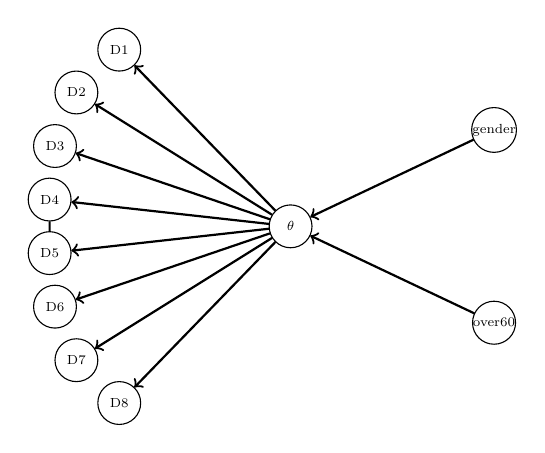
\begin{tikzpicture}[scale=0.68,transform shape,
  every node/.style={font=\scriptsize}]

% Items, placed on a left arc
\node[nodecircle] (D1) at (-3.2,  2.8) {D1};
\node[nodecircle] (D2) at (-4.0,  2.0) {D2};
\node[nodecircle] (D3) at (-4.4,  1.0) {D3};
\node[nodecircle] (D4) at (-4.5,  0.0) {D4};
\node[nodecircle] (D5) at (-4.5, -1.0) {D5};
\node[nodecircle] (D6) at (-4.4, -2.0) {D6};
\node[nodecircle] (D7) at (-4.0, -3.0) {D7};
\node[nodecircle] (D8) at (-3.2, -3.8) {D8};

% Latent variable in the middle
\node[nodecircle] (theta) at (0, -0.5) {$\theta$};

% Exogenous variables on the right
\node[nodecircle] (gender) at (3.8, 1.3) {gender};
\node[nodecircle] (over60) at (3.8,-2.3) {over60};

% Measurement edges
\draw[->,thick] (theta) -- (D1);
\draw[->,thick] (theta) -- (D2);
\draw[->,thick] (theta) -- (D3);
\draw[->,thick] (theta) -- (D4);
\draw[->,thick] (theta) -- (D5);
\draw[->,thick] (theta) -- (D6);
\draw[->,thick] (theta) -- (D7);
\draw[->,thick] (theta) -- (D8);

% Score associations
\draw[dif] (gender) -- (theta);
\draw[dif] (over60) -- (theta);

% Local dependence
\draw[ld] (D4) -- (D5);

\end{tikzpicture}

\vspace{0.3em}
\textbf{(a)}
\end{minipage}
\hfill
% -------------------- (b) Moralized graph --------------------
\begin{minipage}[t]{0.48\textwidth}
\centering
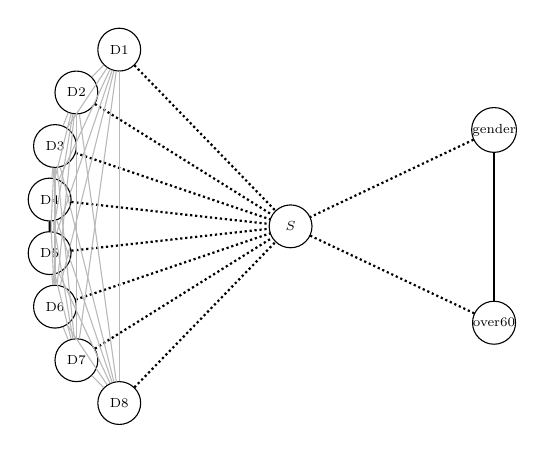
\begin{tikzpicture}[scale=0.68,transform shape,
  every node/.style={font=\scriptsize}]

% Items, placed on a left arc / clique
\node[nodecircle] (D1) at (-3.2,  2.8) {D1};
\node[nodecircle] (D2) at (-4.0,  2.0) {D2};
\node[nodecircle] (D3) at (-4.4,  1.0) {D3};
\node[nodecircle] (D4) at (-4.5,  0.0) {D4};
\node[nodecircle] (D5) at (-4.5, -1.0) {D5};
\node[nodecircle] (D6) at (-4.4, -2.0) {D6};
\node[nodecircle] (D7) at (-4.0, -3.0) {D7};
\node[nodecircle] (D8) at (-3.2, -3.8) {D8};

% Score in the middle
\node[nodecircle] (S) at (0, -0.5) {$S$};

% Exogenous variables on the right
\node[nodecircle] (gender) at (3.8, 1.3) {gender};
\node[nodecircle] (over60) at (3.8,-2.3) {over60};

% Score-item edges
\draw[scoreedge] (D1) -- (S);
\draw[scoreedge] (D2) -- (S);
\draw[scoreedge] (D3) -- (S);
\draw[scoreedge] (D4) -- (S);
\draw[scoreedge] (D5) -- (S);
\draw[scoreedge] (D6) -- (S);
\draw[scoreedge] (D7) -- (S);
\draw[scoreedge] (D8) -- (S);

% Item-score moralization clique
\foreach \i/\j in {
D1/D2,D1/D3,D1/D4,D1/D5,D1/D6,D1/D7,D1/D8,
D2/D3,D2/D4,D2/D5,D2/D6,D2/D7,D2/D8,
D3/D4,D3/D5,D3/D6,D3/D7,D3/D8,
D4/D6,D4/D7,D4/D8,
D5/D6,D5/D7,D5/D8,
D6/D7,D6/D8,
D7/D8}
{
  \draw[thin,gray!55] (\i) -- (\j);
}

% Local dependence, emphasized on top of the moralization edge
\draw[ld] (D4) -- (D5);

% Score associations
\draw[scoreedge] (gender) -- (S);
\draw[scoreedge] (over60) -- (S);

% Moralized parent edge
\draw[ld] (gender) -- (over60);

\end{tikzpicture}

\vspace{0.3em}
\textbf{(b)}
\end{minipage}

\caption{
Disability subscale graphs: (a) IRT graph; (b) corresponding moralized graph.}\label{fig-disabilitygraph}
\end{figure}


\begin{figure}[ht]
\centering

% -------------------- (a) IRT graph --------------------
\begin{minipage}[t]{0.48\textwidth}
\centering
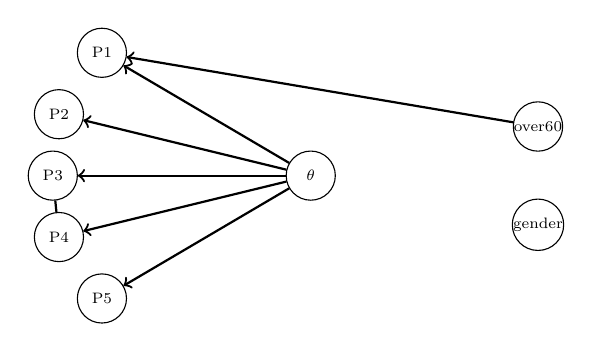
\begin{tikzpicture}[scale=0.78,transform shape,
  every node/.style={font=\scriptsize}]

% Items, placed on a left arc
\node[nodecircle] (P1) at (-3.4,  2.0) {P1};
\node[nodecircle] (P2) at (-4.1,  1.0) {P2};
\node[nodecircle] (P3) at (-4.2,  0.0) {P3};
\node[nodecircle] (P4) at (-4.1, -1.0) {P4};
\node[nodecircle] (P5) at (-3.4, -2.0) {P5};

% Latent variable in the middle
\node[nodecircle] (theta) at (0, 0) {$\theta$};

% Exogenous variable on the right
\node[nodecircle] (over60) at (3.7, 0.8) {over60};
\node[nodecircle] (age) at (3.7, -0.8) {gender};

% Measurement edges
\draw[->,thick] (theta) -- (P1);
\draw[->,thick] (theta) -- (P2);
\draw[->,thick] (theta) -- (P3);
\draw[->,thick] (theta) -- (P4);
\draw[->,thick] (theta) -- (P5);

% DIF edge
\draw[dif] (over60) -- (P1);

% Local dependence
\draw[ld] (P3) -- (P4);

\end{tikzpicture}

\vspace{0.3em}
\textbf{(a)}
\end{minipage}
\hfill
% -------------------- (b) Moralized graph --------------------
\begin{minipage}[t]{0.48\textwidth}
\centering
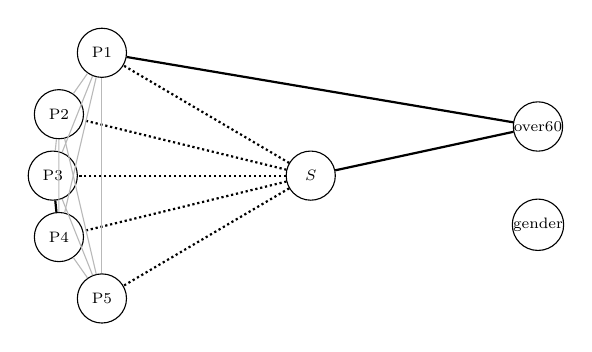
\begin{tikzpicture}[scale=0.78,transform shape,
  every node/.style={font=\scriptsize}]

% Items, placed on a left arc / clique
\node[nodecircle] (P1) at (-3.4,  2.0) {P1};
\node[nodecircle] (P2) at (-4.1,  1.0) {P2};
\node[nodecircle] (P3) at (-4.2,  0.0) {P3};
\node[nodecircle] (P4) at (-4.1, -1.0) {P4};
\node[nodecircle] (P5) at (-3.4, -2.0) {P5};

% Score node in the middle; named S in TikZ, displayed as #
\node[nodecircle] (Score) at (0, 0) {$S$};

% Exogenous variable on the right
\node[nodecircle] (over60) at (3.7, 0.8) {over60};
\node[nodecircle] (age) at (3.7, -0.8) {gender};

% Score-item edges
\draw[scoreedge] (Score) -- (P1);
\draw[scoreedge] (Score) -- (P2);
\draw[scoreedge] (Score) -- (P3);
\draw[scoreedge] (Score) -- (P4);
\draw[scoreedge] (Score) -- (P5);

% Item-score moralization clique
\foreach \i/\j in {
P1/P2,P1/P3,P1/P4,P1/P5,
P2/P3,P2/P4,P2/P5,
P3/P5,
P4/P5}
{
  \draw[thin,gray!55] (\i) -- (\j);
}

% Local dependence, emphasized on top of the moralization edge
\draw[ld] (P3) -- (P4);

% DIF edge in the moralized graph
\draw[ld] (over60) -- (P1);

% Moralized parent edge
\draw[ld] (Score) -- (over60);

\end{tikzpicture}

\vspace{0.3em}
\textbf{(b)}
\end{minipage}

\caption{
Pain subscale graphs: (a) IRT graph; (b) corresponding moralized graph.
}\label{fig-paingraph}
\end{figure}


\subsection{Step 6}
Step 6 retests the retained DIF and LD edges using the conditioning sets implied by the graphs. For these two subscales, the LD and DIF structures make the additional tests redundant. The final graphs are therefore those reported in Step 5 (Figures~\ref{fig-disabilitygraph} and~\ref{fig-paingraph}).



\end{appendices}


\end{document}
